\documentclass[
	12pt,				% tamanho da fonte
	oneside,			% para impressão em recto e verso. Oposto a oneside
	a4paper,			% tamanho do papel. 
	english,			% idioma adicional para hifenização
	brazil,				% o último idioma é o principal do documento
	]{abntex2}

% ---
% Pacotes fundamentais 
% ---
\usepackage{lmodern}			% Usa a fonte Latin Modern
\usepackage[T1]{fontenc}		% Selecao de codigos de fonte.
\usepackage[utf8]{inputenc}		% Codificacao do documento (conversão automática dos acentos)
\usepackage{indentfirst}		% Indenta o primeiro parágrafo de cada seção.
\usepackage{color}				% Controle das cores
\usepackage{graphicx}			% Inclusão de gráficos
\usepackage{microtype} 			% para melhorias de justificação
\usepackage{multicol}
\usepackage{multirow}
\usepackage[brazilian,hyperpageref]{backref}	 % Paginas com as citações na bibl
\usepackage[alf]{abntex2cite}	% Citações padrão ABNT
\usepackage{listings}
\usepackage{float}

\lstset{
  showspaces=false,
  showtabs=false,
  breaklines=true,
  showstringspaces=false,
  breakatwhitespace=true,
  commentstyle=\color{green},
  keywordstyle=\color{blue},
  stringstyle=\color{red},
  basicstyle=\ttfamily
}

% --- 
% CONFIGURAÇÕES DE PACOTES
% --- 

% ---
% Configurações do pacote backref
% Usado sem a opção hyperpageref de backref
\renewcommand{\backrefpagesname}{Citado na(s) página(s):~}
% Texto padrão antes do número das páginas
\renewcommand{\backref}{}
% Define os textos da citação
\renewcommand*{\backrefalt}[4]{
	\ifcase #1 %
		Nenhuma citação no texto.%
	\or
		Citado na página #2.%
	\else
		Citado #1 vezes nas páginas #2.%
	\fi}%
% ---

% ---
% Informações de dados para CAPA e FOLHA DE ROSTO
% ---
\titulo{Prática 4: Restaurante(Threads)}
\autor{Pedro Inácio Rodrigues Pontes}
\local{Belo Horizonte, Brasil}
\data{2025}
\instituicao{%
  Universidade Federal de Minas Gerais
  \par
  Colégio Técnico
  \par
  Curso Técnico em Desenvolvimento de Sistemas}

\definecolor{blue}{RGB}{41,5,195}

\makeatletter
\hypersetup{
     	%pagebackref=true,
		pdftitle={\@title}, 
		pdfauthor={\@author},
    	pdfsubject={\imprimirpreambulo},
		colorlinks=true,       		% false: boxed links; true: colored links
    	linkcolor=blue,          	% color of internal links
    	citecolor=blue,        		% color of links to bibliography
    	filecolor=magenta,      		% color of file links
		urlcolor=blue,
		bookmarksdepth=4
}
\makeatother

\renewcommand{\thesection}{\arabic{section}}
\setlength{\parindent}{1.3cm}
\setlength{\parskip}{0.2cm} 

\makeindex


\begin{document}

\selectlanguage{brazil}
\frenchspacing 

\imprimircapa

{
\ABNTEXchapterfont

\textual

% ----------------------------------------------------------
% Introdução (exemplo de capítulo sem numeração, mas presente no Sumário)
% ----------------------------------------------------------
\section{Introdução}

O objetivo da presente prática foi reproduzir a lógica de um restaurante, com chefs e garçons, implementando estes em forma de threads, assim aplicando seus conceitos. Foi pedida a criação de três tipos diferentes de pratos, de ingredientes, que são produzidos por porções, de chamadas aleatórias de pedidos a partir do garçom e preparação destes pelo chef.

\section{Desenvolvimento}

Para estruturar o "Restaurante", foram criadas diversas classes com funções de estruturar o código. Tal poderia ser feito apenas em uma classe Program, mas ficaria menos robusto, assim, este código possui uma estrutura sólida que permite expansão rápida e simples da sua lógica, mesmo que tal estrutura tenha sido bem mais demorada para fazer.

O código possui 8 classes:
\begin{enumerate}
    \item Ingredient
    \item TypeDish
    \item IngredientsStock
    \item Order
    \item ConsoleLock
    \item Waiter
    \item Chef
    \item Program (main)
\end{enumerate}

\subsection{Classes Enum}
Ingredient é uma classe tipo enum, a qual possui instâncias fixas que seriam os tipos do enum, além de suas propriedades extras: PreparationTime, PortionsByPreparation, Order (para ordenar as instâncias fixas da classe, isso serve para evitar deadlocks numa lógica posterior), Name. Serve para organização forte dos ingredientes.

TypeDish é outra classe tipo enum, que possui instâncias fixas dos pratos, mais um dicionário com o nome dos ingredientes usados e suas quantidades.

Estrutura básica de uma classe enum (exemplo de Ingredient):

\begin{lstlisting}
public class Ingredient
{
    private static int _nextOrder = 0;

    public int Order {get;}
    public int PreparationTime { get; }
    public int PortionsByPreparation { get; }
    public string Name { get; }

    private static readonly ConcurrentDictionary<string, Ingredient> _types;

    static Ingredient()
    {
        _types = new ConcurrentDictionary<string, Ingredient>();

        Arroz = new Ingredient("Arroz", 3);
        Macarrao = new Ingredient("Macarrao", 4);
        Molho = new Ingredient("Molho", 2);
        Carne = new Ingredient("Carne", 2);
    }

    private Ingredient(string name, int portionsByPreparation)
    {
        Name = name;
        PortionsByPreparation = portionsByPreparation;
        PreparationTime = portionsByPreparation * 2;
        Order = _nextOrder++;

        _types[name] = this;
    }

    public static readonly Ingredient Arroz;
    [...]
\end{lstlisting}

\subsection{Lógica dos Pedidos}
IngredientsStock armazena um dicionário com um objeto Ingredient e sua quantidade, além de um dicionário para os locks do ingrediente <Ingredient, Object>. Ela possui os seguintes métodos:

\begin{lstlisting}
    public bool HasSuficientStock(TypeDish dish)
    public Dictionary<Ingredient, int> ConsumeIngredient(TypeDish dish)
    public void AddIngredient(Ingredient ingredient, int amount)
    private IEnumerable<KeyValuePair<Ingredient, int>> GetOrderedIngredients(TypeDish dish)
\end{lstlisting}

ConsumeIngredient retorna os ingredientes que estão faltando para o prato se o estoque for menor que a quantidade necessária, e a suas quantidades necessárias. GetOrderedIngredients ordena os ingredientes de forma fixa baseada no atributor Order de Ingredient para manter uma ordem fixa de retorno. Isso evita que sejam feitos deadlocks quando é feito um lock para cada ingrediente que será verificado ou consumido no prato. Veja o código de HasSufucientStock para perceber a necessidade dessa ordenação para evitar um deadlock ao verificar dois pratos diferentes simultaneamente:

\begin{lstlisting}
public bool HasSuficientStock(TypeDish dish)
{
    foreach (var (ingredient, quantity) in GetOrderedIngredients(dish))
    {
        lock (_locks[ingredient])
        {
            if (Stock[ingredient] < quantity)
                return false;
        }
    }
    return true;
}
\end{lstlisting}

Order armazena o prato desejado e seu id que é autoincrementado por \textit{Interlocked.Increment()}. Também possui um ToString para descrever esses dois atributos no console.

\subsection{ConsoleLock}

ConsoleLock é uma classe criada para escrever as mensagens no console suportando as threads sem erro, já que possui um lock global, assim só uma thread pode a acessar por vez. Também define a cor do log como parâmetro

\subsection{Lógica Final}

Waiter tem recebe uma BlockingCollection ordersQueue que é compartilhada com chef. Ela armazena a fila de pedidos. Seu código principal é relativamente simples e autoexplicativo:

\begin{lstlisting}
public void Start() {
    Task.Run(() =>
    {
        while(true)
        {
            try
            {
                int waitTime = _random.Next(1_000, 10_001);
                Thread.Sleep(waitTime);
                var selectedDish = TypeDish.All[_random.Next(TypeDish.All.Count)];
                var order = new Order(selectedDish);
                _ordersQueue.Add(order);
                ConsoleLock.Log(ConsoleColor.Blue, $"[Garçom {_name}] - Envio de {order}");
            }
            catch(Exception e)
            {
                ConsoleLock.Log(ConsoleColor.DarkRed, $"[{_name}] - ERRO: {e.Message}");
            }
        }
    });
}
\end{lstlisting}

Chef também possui o metódo Start, além dos métodos auxiliares:
\begin{lstlisting}
    private void ProcessOrder(Order order)
    private int CalculatePortionsToProduce(int missingAmount, int portionsByPreparation)
    private void PrepareIngredient(Ingredient ingredient, int portions)
    private void AssembleDish(Order order)
\end{lstlisting}

AssembleDish, o método menos descritivo, cuida do tempo de montagem dos pratos a partir do número ingredientes utilizados.

Os métodos centrais de chef, Start e ProcessOrder, seguem abaixo:
\begin{lstlisting}
public void Start()
{
    Task.Run(() =>
    {
        while (true)
        {
            try
            {
                var order = _ordersQueue.Take();
                ProcessOrder(order);
            }
            catch (Exception e)
            {
                ConsoleLock.Log(ConsoleColor.DarkRed, $"[{_name}] - ERRO: {e.Message}");
            }
        }
    });
}

private void ProcessOrder(Order order)
{
    Dictionary<Ingredient, int> missingIngredients = _stock.ConsumeIngredient(order.Dish);
    ConsoleLock.Log(ConsoleColor.DarkRed, $"[Chef {_name}] - Inicio da Preparacao do Pedido {order.Id}");
    foreach (var (ingredient, missingAmount) in missingIngredients)
    {
        int portionsToProduce = CalculatePortionsToProduce(missingAmount, ingredient.PortionsByPreparation);
        PrepareIngredient(ingredient, portionsToProduce);
    }
    AssembleDish(order);
    ConsoleLock.Log(ConsoleColor.DarkRed, $"[Chef {_name}] - Fim da Preparação do Pedido {order.Id}");
}
\end{lstlisting}

A classe Program cuida da montagem correta do programa após toda a sua definição lógica. Ela é enxuta é está definida com:
\begin{lstlisting}
class Program
{
    static void Main(string[] args)
    {
        BlockingCollection<Order> ordersQueue = new();
        IngredientsStock stock = new();
        
        List<string> chefNames = new(){"Quaresma", "Reinaldo", "Jorge"};
        List<string> waiterNames = new(){"Rodrigo", "Sergio", "Alemão", "Mafeus", "LP"};

        Chef[] chefs = new Chef[3];
        Waiter[] waiters = new Waiter[5];

        for (int i = 0; i < 5; i++)
        {
            waiters[i] = new Waiter(waiterNames[i], ordersQueue);
            waiters[i].Start();
        }

        for (int i = 0; i < 3; i++)
        {
            chefs[i] = new Chef(chefNames[i], ordersQueue, stock);
            chefs[i].Start();
        }

        Console.ReadLine();
    }
}
\end{lstlisting}

\section{Resultados}

Veja que os pedidos são feitos e preparados paralelamente, com um prato deixando de ser feito paralelamente apenas quando outro chef está utilizando um de seus ingredientes.

\begin{figure}[H]
    \centering
    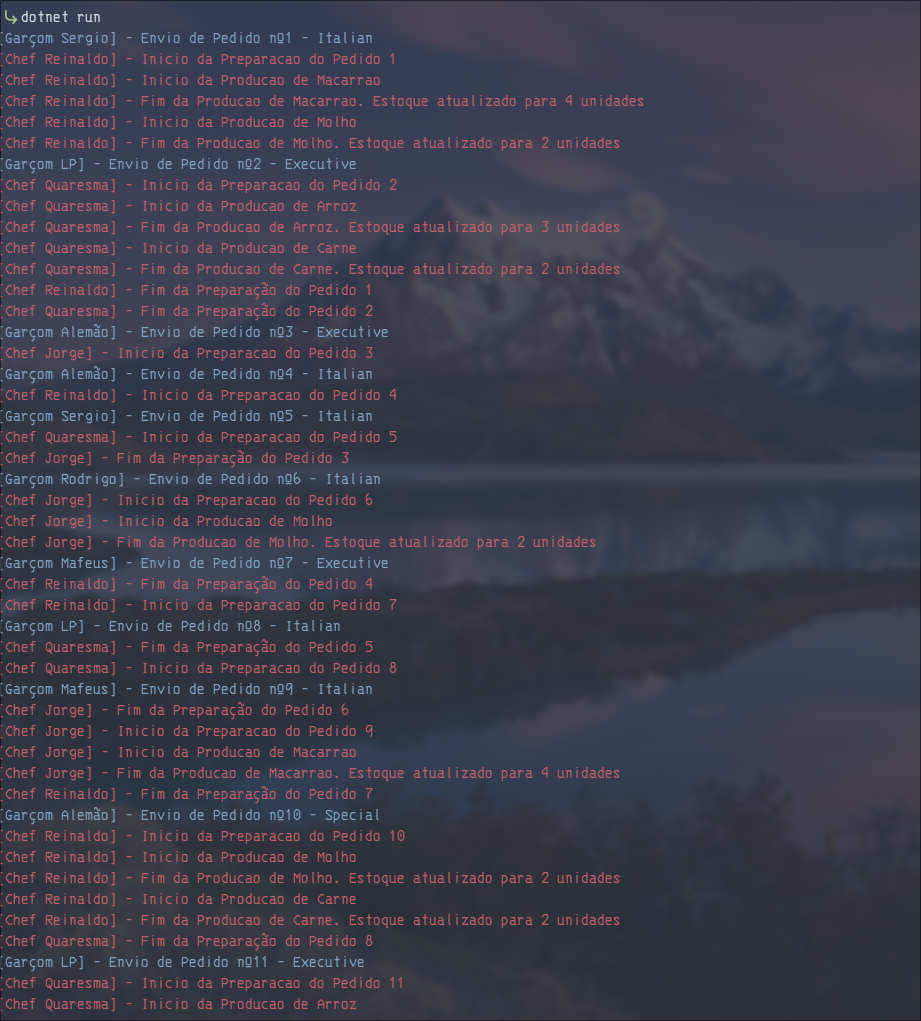
\includegraphics[width=0.7\textwidth]{img1.png}
    \caption{Prorgama Rodando}
    \label{fig:img1}
\end{figure}
\section{Conclusão}

Todos os resultados foram alcançados, e a montagem por classes trouxe os devidos benefícios prometidos, fazendo com que a expansão do código em mais lógica ou mais processamento interno (mais chefs, pratos, ingredientes...) seja simples e fácil.

\end{document}
